\documentclass[letter]{article}
\usepackage[monocolor]{../math232/ahsansabit}
\usepackage[]{tikz}
\usepackage[]{pgfplots}
\title{Classical Mechanics : : Homework 03}
\author{Ahmed Saad Sabit, Rice University}
\date{\today}
 \usepackage[]{float}
\begin{document}
\maketitle
\tableofcontents 
\newpage 
\section{Problem 01} 
\subsection{a}
There are two key points. 
\begin{itemize}
	\item From the given equation in the problem it seems like we have to consider the momentum exchange between resting tiny droplets and bigger raindrop is negligible. Other wise we have to add a $- \lambda \pi r^2 v^2$ term with the effective force. 
	\item Air drag is neglected, as mentioned.
\end{itemize}
The equation of motion hence
\[
F = \frac{\mathrm{d} p}{\mathrm{d} t} = v \frac{\mathrm{d} m}{\mathrm{d} t} + m \frac{\mathrm{d} v}{\mathrm{d} t}
\] 
The only force acting on this waterdrop is $mg$ if we consider positive to point downwards. Hence
\[
\boxed{
mg = v \frac{\mathrm{d} m}{\mathrm{d} t} + m \frac{\mathrm{d} v}{\mathrm{d} t}
}
\]

\newpage 
\subsection{b}
To compute the area swept by the spherical raindrop, we assume $\delta t \neq 0 $ but $\delta t \to  0$. Then the infinitesimal volume swept in that time period, 
\[
\mathrm{d} \nu = 	\left(\pi r^2\right) \left(v \delta t\right)
\]
Let $n$ volume of water be stored per unit volume of air as cloud (this the fraction of the volume taken by the water of droplets in a unit cube of air). So the amount of mist/water/fog in the swept region is
\[
 n \mathrm{d} \nu = \mathrm{d} V = n \pi r^2 v \delta t 
\]
As stated in the problem, the raindrop holds its spherical shape and absorbs this volume of water. As water is incompressible, this adds to the volume of the raindrop. Hence, the rate of increase of volume of the raindrop is 
\[
	\frac{\mathrm{d} V}{\mathrm{d} t} = n \pi r^2 v
\]
From this we can compute rate of change of radius easily 
\begin{align*}
	\frac{\mathrm{d} }{\mathrm{d} t} \left(\frac{4}{3} \pi r^3\right) &= n \pi r^2 v \\
	(4 \pi r^2 )\frac{\mathrm{d} r}{\mathrm{d} t}&= n \pi r^2 v \\
	\frac{\mathrm{d} r}{\mathrm{d} t} &= \frac{n}{4} v \equiv \eta v
\end{align*}
Hence 
\[
\boxed{
\eta = \frac{n}{4}
}
\] 
\textbf{NOTE} We can show that $n = \frac{\rho_{\text{fog}}}{\rho_w}$ pretty easily. 
$n$ is the amount of water in unit volume of air in the form of mist/cloud/fog. Let density of overall amount of water in the form of cloud be $\rho_f$, then total mass of the water is 
\[
m_w = \rho_w v = \rho_f V
\]
$v$ is the volume of water if all the cloud was condensed, $V$ is the volume of the overall cloud. We can see, the fraction of volume of water occupied per unit volume in the air as cloud, 
\[
\frac{v}{V} = n = \frac{\rho_f}{\rho_w}
\]
So we can also have written $ \eta = \frac{1}{4} \frac{\rho_f}{\rho_w}$

\newpage 
\subsection{c} 
Mass derivative \[
\frac{\mathrm{d} m}{ \mathrm{d} t} = \rho \frac{\mathrm{d} V}{\mathrm{d} t} = \rho n \pi r^2 v
\]
Now using the force equation found in  \textbf{a}
\begin{align*}
	mg &= v \frac{\mathrm{d} m}{\mathrm{d} t} + m \frac{\mathrm{d} v}{\mathrm{d} t}\\
	g &= v \frac{\rho n \pi r^2 v}{m} + \frac{\mathrm{d} v}{\mathrm{d} t} \\
	g &= v \frac{(m) n \pi r^2 v}{ (( 4 / 3) \pi r^3) m } + \frac{\mathrm{d} v}{\mathrm{d} t} \\
	g &= v^2 \left(\frac{3n}{4r}\right) + \frac{\mathrm{d} v}{\mathrm{d} t} 
\end{align*}
Hence the time derivative dependency is found. We need to eliminate $t$ at some point. 
\[
	r \frac{\mathrm{d} v}{\mathrm{d} t} + \left(\frac{3n}{4}\right) v^2 - rg = 0
\] 

Using $\mathrm{d} r / \mathrm{d} t$ 
\[
\frac{\mathrm{d} r}{\mathrm{d} t} = \frac{n}{4} v
\]
the acceleration can be re-written as 
\[
\frac{\mathrm{d} v}{\mathrm{d} t} = 
\frac{\mathrm{d} v}{\mathrm{d} r} \frac{\mathrm{d} r}{\mathrm{d} t} 
= \frac{\mathrm{d} v}{\mathrm{d} r} \frac{n}{4} v  = \left(\frac{1}{2} \frac{\mathrm{d} v^2}{\mathrm{d} r}\right) \frac{n}{4} = \frac{n}{8} \frac{\mathrm{d} (v^2 )}{\mathrm{d} t}
\] 
The computational trick I use here, 
\[
v \frac{\mathrm{d} v}{\mathrm{d} r} = \frac{v \, \mathrm{d} v}{\mathrm{d}  r} = 
\frac{d \left( \int v \mathrm{d} v\right)}{\mathrm{d}  r} = 
\frac{d \left(\frac{1}{2} v^2 \right)}{ \mathrm{d} r} = \frac{1}{2} \frac{\mathrm{d} v^2}{\mathrm{d} r}
\] 
\[
	\frac{nr}{8} \frac{\mathrm{d} (v^2)}{\mathrm{d} r} + \left(\frac{3n}{4}\right) v^2 - rg = 0
\]
\[
\boxed{
\frac{\mathrm{d} (v^2)}{\mathrm{d} r} + \frac{6}{r} v^2 - \frac{8}{n} g = 0
}\]
If you, dear Grader, prefer $\eta$, 
\[
\boxed{
\frac{\mathrm{d} (v^2)}{\mathrm{d} r} + \frac{6}{r} v^2 - \frac{2}{\eta } g = 0
}
\]
\newpage 
\subsection{d} 
We can re-write above equation as 
\[
\frac{1}{2} v \frac{\mathrm{d} v}{\mathrm{d} r} + \frac{6}{r} v^2 - \frac{8}{n} g = 0
\]
Introducing $\eta  = n / 4$ and doing an algebraic re-write 
\[
	\frac{\mathrm{d} v}{\mathrm{d} r} = \frac{g}{\eta v}  - \frac{3v}{r}
\]
We do this to write a power law solution. Assuming $v(r) = Ar^{n}$ (power $n$ not to be confused with amount of fog) we have
\[
\frac{\mathrm{d} v}{\mathrm{d} r} = n A r^{n-1}
\]
Henceforth 
\[
n A r^{n- 1} = \frac{g}{\eta A r^{n} } - \frac{3 A r^{n}}{r}
\]
\[
	(n A + 3A) r^{n-1} = \frac{g}{\eta A r^{n}}
\] 
\[
	(n+3) A r^{2n - 1} = \frac{g}{\eta A}
\] 
So this means that 
\[
r^{2n - 1} = 1 = r ^{0}
\] 
Hence $ n = \frac{1}{2}$. If we solve for $A$ here now, 
\[
\frac{7}{2} A = \frac{g}{\eta A} 
\]
Which gives us 
\[
\boxed{
A = \sqrt{\frac{2g}{7 \eta}} 
}\]
So the solution leaves us with 
\[\boxed{
v(r) = \sqrt{\frac{2g}{7 \eta} r} 
}\]
Now we can proceed to find the time dependence relations. $v(r) = A r^{n}$. 
\[
\frac{\mathrm{d} v}{\mathrm{d} t} = \frac{1}{2} A r^{-\frac{1}{2}} \frac{\mathrm{d} r}{\mathrm{d} t}	= 
\frac{1}{2} A r^{- 1 / 2} \eta v
\]
But $r = \frac{v(r)^2}{A^2}$ hence, 
\[
\frac{\mathrm{d} v}{\mathrm{d} t} = \frac{1}{2} A \frac{A}{v} \eta v = \frac{1}{2} A^2 \eta
\]
Henceforth, 
\[
\boxed{
v(t) = \frac{1}{2} A^2 \eta t }
\]
Similarly, 
\[
	\frac{\mathrm{d} r}{\mathrm{d} t} = \eta \left(\frac{1}{2} A^2 \eta t\right)
\]
\[
\boxed{
r(t) = \frac{1}{4} A^{2} \eta^2 t^2
}
\] 
For the mass rate, 
\[
\frac{\mathrm{d} m}{ \mathrm{d} t} = \rho_w n \pi r ^2 v  
\]
Substituting the formulas we found for $r(t) $ and $v(t)$ and taking a simple integral we find, 
\[
m = \frac{1}{192} \rho_w n A^{6} \eta ^{5} t ^{6} 
\]
\[
\rho_w n = 4 \rho_w \eta \to \frac{1}{48} \rho_w A ^{6} \eta ^{6} t ^{6}  
\]
\[
\boxed{
m(t) = \frac{1}{48} \rho_w A^{6} \eta ^{6} t ^{6}
}
\]
\newpage 
\subsection{e} 
With the euphemism of $v^2 = x$ we can re-write the differential equation we found earlier, 
\[
v^2 = x
\] 
\[
\boxed{
\frac{\mathrm{d} x}{\mathrm{d} r} + \frac{6x}{r} - \frac{8g}{n} = 0
}
\] 
\
\begin{tcolorbox}[colback=white,colframe=gray,sharp corners]
	\textbf{Solving the above differential equation: }
This is a standard differential equation that can be crunched with integrating factor method (MATH 211)
\[
\frac{dx}{dr} + P(r)x = Q(r)
\]
Here, \( P(r) = \frac{6}{r} \) and \( Q(r) = \frac{8g}{n} \).
The integrating factor \( \mu(r) \) is given by:

\[
\mu(r) = e^{\int P(r) dr} = e^{\int \frac{6}{r} dr} = e^{6 \ln r} = r^6
\]
Multiplying the factor
\[
r^6 \frac{dx}{dr} + 6r^5x = \frac{8g}{n} r^6
\]
The left-hand side is the derivative of \( r^6x \), so:
\[
\frac{d}{dr}(r^6x) = \frac{8g}{n}r^6
\]
\[
r^6x = \int \frac{8g}{n}r^6 dr
\]
\[
r^6x = \frac{8g}{n} \cdot \frac{r^7}{7} + C = \frac{8g}{7n}r^7 + C
\]
\[
x(r) = \frac{8g}{7n}r + \frac{C}{r^6}
\]
We can solve from $C$ from boundary conditions 
\[
\boxed{
v^2 (r) = \frac{8g}{7n} r + \frac{C}{r^{6}}
}
\]
Using $ \eta = \frac{n}{4}$ we can also do a re-write, 
\[
\boxed{
v^2(r) = \frac{2g}{7 \eta }r + \frac{C}{r^{6}}
}
\] 
\end{tcolorbox}
So what we have is 
\[
v(r) = \sqrt{\frac{2g}{7 \eta} r + \frac{C}{r^{6}}} 
\]
This gives us $\mathrm{d} r / \mathrm{d} t$ purely in terms of $r$. 
\[
\frac{\mathrm{d} r}{\mathrm{d} t} = \eta 
 \sqrt{\frac{2g}{7 \eta} r + \frac{C}{r^{6}}} 
\] 
We know that for relatively normal $r$ we have $\frac{1}{r^{6}} $ be insanely small. This term would rather vanish when compared to linearly increasing $\frac{2g}{7 \eta} r$.

\begin{center}
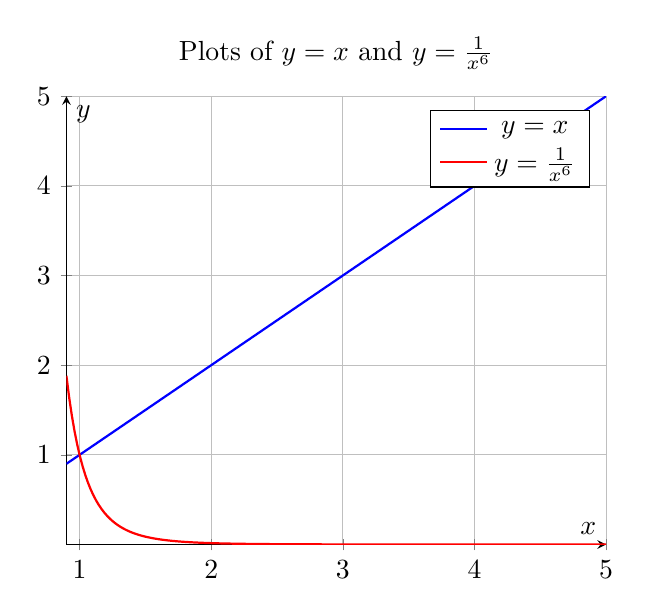
\begin{tikzpicture}
    \begin{axis}[
        xlabel={$x$},
        ylabel={$y$},
        title={Plots of $y = x$ and $y = \frac{1}{x^6}$},
        legend pos=north east,
        grid=major,
        domain=0.9:5,
        samples=200,
        axis lines=middle
    ]
    % Plot y = x
    \addplot[color=blue, thick]{x};
    \addlegendentry{$y = x$};
    
    \addplot[color=red, thick]{1/x^6};
    \addlegendentry{$y = \frac{1}{x^6}$};
    
    \end{axis}
\end{tikzpicture}
\end{center}
Linearity dominates, obviously. Hence a good approximation we can be left with is, 
\[
v(r) \approx \sqrt{\frac{2g}{7 \eta } r}  = A \sqrt{r} 
\] 
Which perfectly aligns with our power-law solution. 
\newpage
	\section{Problem 02} 

	Consider a position $r \in  [x,  x + \mathrm{d} x]$. A particle stays in this region for $\mathrm{d} t_{1 / 2 } = \frac{\mathrm{d} x}{v(x)}$ time for half period of motion, and $ \mathrm{d} t = 2 \frac{\mathrm{d} x}{v(x)}$ for full period of motion. We can make symmetry assumptions because the motion is given to be simple harmonic. 
	The probability is defined in a manner
	\[
	P(x) \mathrm{d} x = \frac{\mathrm{d} t}{\tau} = \frac{2}{\tau v(x)} \mathrm{d} x 
	\]
	\[
	\boxed{
	P(x) = \frac{2}{\tau v(x)}
	}
	\] Where $\tau$ is the full period of motion.

	Solution for $v(x)$ in case of simple harmonic motion 
	\[
		v(x) = \sqrt{\frac{2E}{m} - \frac{k}{m} x^2}  \]
	\[
	\tau = 2 \pi \sqrt{\frac{m}{k}} 
	\]
	\[
	P(x) = \frac{2}{2 \pi \sqrt{\frac{2E}{k} - x^2} } = \frac{1}{ \pi \sqrt{\frac{2E}{k} - x^2} }
	\]

	We can test whether our probability is normalize, as $x \in \left[-\sqrt{  \frac{2E}{k}}, \sqrt{ \frac{2E}{k} } \right]$. We can also change our notation to be more convenient $\frac{2E}{k} = A^2$ which is the amplitude, 
	\[
	\int_{-A}^{A} P(x) \, \mathrm{d} x =  \int_{-A}^{A} \frac{\mathrm{d}  x}{\pi \sqrt{A^2 - x^2} } = 1 
	\] 
	This gives us 
	\[
	\boxed{
	P(x) = \frac{1}{\pi \sqrt{A^2 - x^2} }
	}
	\] 

	\begin{figure}[H]
		\centering
		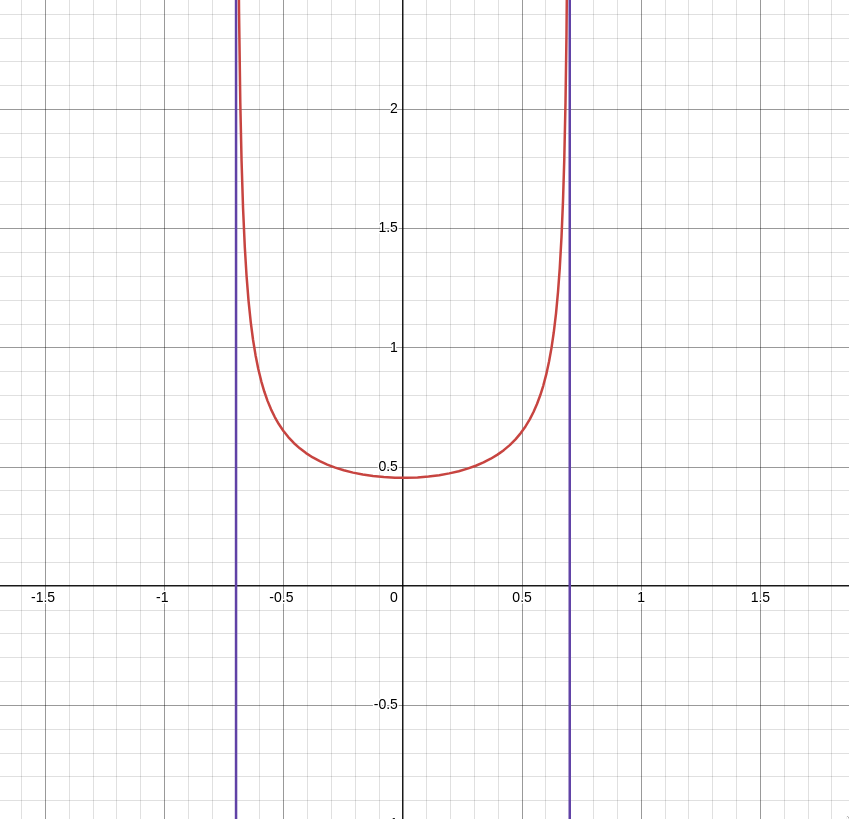
\includegraphics[width=0.5\textwidth]{ss/ncl01.png}
		\caption{Vertical lines represent boundary}
		\label{fig:ss-ncl01-png}
	\end{figure}
	The infinity at $x = A$ and $x = -A$ makes sense because $v(x) = 0$ and the time it stays in that position is indefinite. But physically we know that the particle spends infinitesimally small amount of time in that position as  of the spring force, so we can safely neglect the boundary blowing up. 

	More pure mathematically, we only are interested on the area under the curve (integral) for the probability. The $x = A$ and $x = -A$ region is content zero, so we still can take the integral under the curve without any difficulty even after having infinity there.  
	\begin{figure}[H]
		\centering
		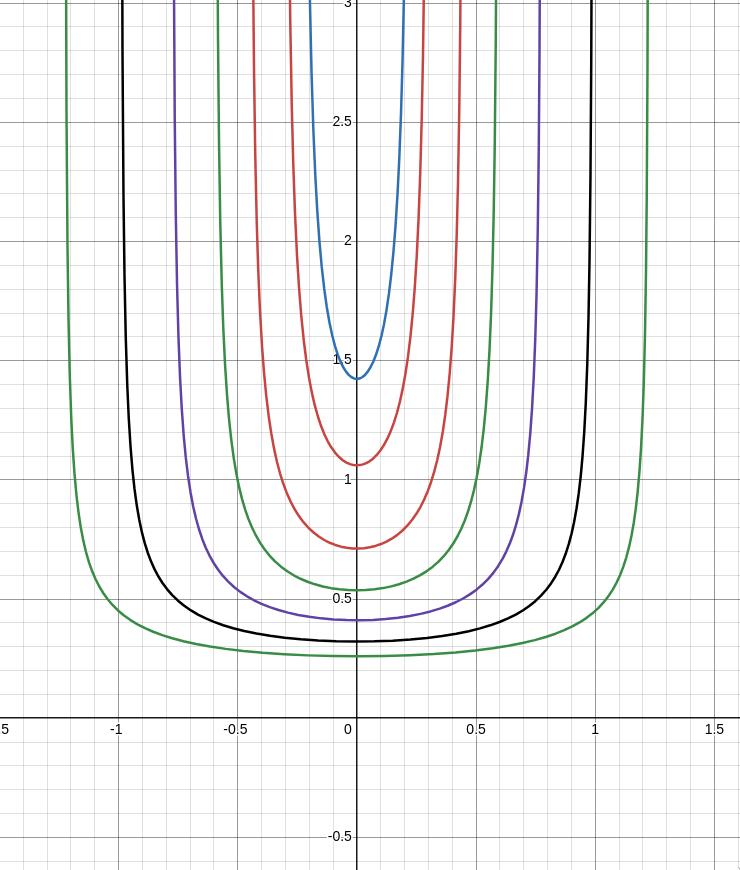
\includegraphics[width=0.5\textwidth]{ss/ncl02.png}
		\caption{Various plots for various amplitudes}
		\label{fig:ss-ncl01-png}
	\end{figure}

	This makes perfect sense because the lowest probability of time spent in the center aligns with the graph, as the speed is maximum there. The area under each and every single curve is going to be 1 for normalization, and regions under the graph in general describe probability of finding the particle there. Note this region $R$ must be such that $R \subset [-A,A]$. 

\begin{figure}[H]
	\centering
	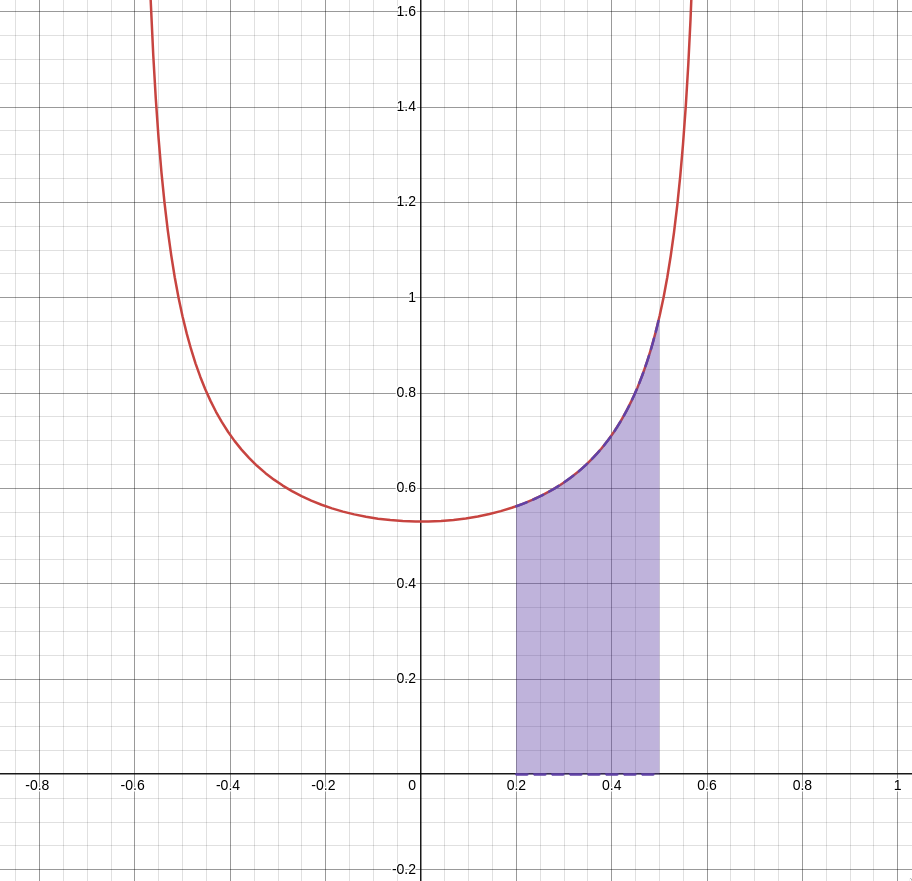
\includegraphics[width=0.5\textwidth]{ss/ncl03.png}
	\caption{Probability of finding a particle in given $x$ region is the area. I did the calculation it shows 0.23 something, so like 23\%.}
	\label{fig:ss-ncl03-png}
\end{figure}

\newpage
\section{Problem 03} 
I did that by hand. I'd rather upload it in it's pure form. I know it is an eye-sore, but I don't know how to draw it properly on the computer. 
\end{document}
